% Standalone source of the architecture figure. Compiled to figures/arch_dacshed.pdf
% and included by the manuscript, because TikZ cannot be loaded inside the sn-jnl class here.
\documentclass[border=2pt]{standalone}
\usepackage{amsmath}
\usepackage{tikz}
\usetikzlibrary{arrows.meta,positioning,shapes.geometric,fit,calc}
\begin{document}
\scalebox{1.4}{%
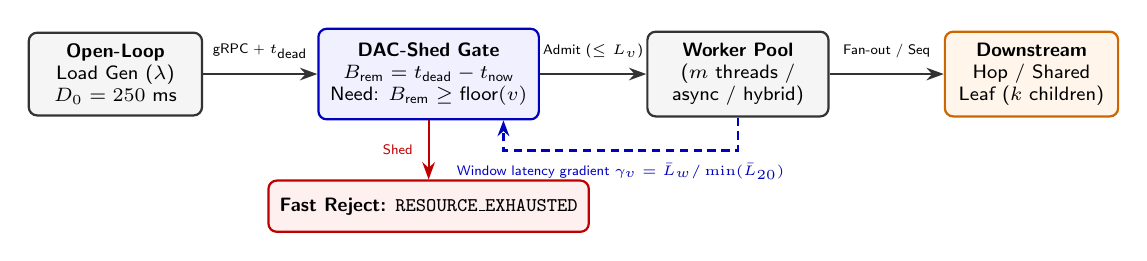
\begin{tikzpicture}[
    font=\sffamily\scriptsize,
    box/.style={draw=black!80, rounded corners=3pt, thick, align=center, minimum height=1.05cm, fill=gray!8, inner sep=4pt},
    gate/.style={draw=blue!75!black, rounded corners=3pt, thick, align=center, minimum height=1.15cm, fill=blue!6, inner sep=4pt},
    leaf/.style={draw=orange!80!black, rounded corners=3pt, thick, align=center, minimum height=1.05cm, fill=orange!8, inner sep=4pt},
    reject/.style={draw=red!75!black, fill=red!6, rounded corners=3pt, thick, align=center, minimum height=0.65cm, inner sep=4pt},
    arr/.style={-{Stealth[length=2.2mm, width=1.6mm]}, thick, draw=black!80},
    dasharr/.style={-{Stealth[length=2.0mm, width=1.5mm]}, densely dashed, thick, draw=blue!75!black}
]
\node[box, minimum width=2.2cm] (loadgen) {\textbf{Open-Loop}\\Load Gen ($\lambda$)\\$D_0 = 250\text{ ms}$};
\node[gate, right=1.45cm of loadgen, minimum width=2.8cm] (dac) {\textbf{DAC-Shed Gate}\\$B_{\text{rem}} = t_{\text{dead}} - t_{\text{now}}$\\Need: $B_{\text{rem}} \ge \text{floor}(v)$};
\node[box, right=1.35cm of dac, minimum width=2.3cm] (pool) {\textbf{Worker Pool}\\($m$ threads /\\async / hybrid)};
\node[leaf, right=1.45cm of pool, minimum width=2.2cm] (child) {\textbf{Downstream}\\Hop / Shared\\Leaf ($k$ children)};
\draw[arr] (loadgen.east) -- node[above=2pt, font=\sffamily\tiny] {gRPC + $t_{\text{dead}}$} (dac.west);
\draw[arr] (dac.east) -- node[above=2pt, font=\sffamily\tiny] {Admit ($\le L_v$)} (pool.west);
\draw[arr] (pool.east) -- node[above=2pt, font=\sffamily\tiny] {Fan-out / Seq} (child.west);
\node[reject, below=0.75cm of dac, minimum width=3.1cm] (shed) {\textbf{Fast Reject:} \texttt{RESOURCE\_EXHAUSTED}};
\draw[arr, draw=red!75!black] (dac.south) -- node[left=2pt, font=\sffamily\tiny, text=red!75!black] {Shed} (shed.north);
\draw[dasharr] (pool.south) -- ++(0,-0.42cm) -| ([xshift=0.95cm]dac.south)
    node[pos=0.25, below=1pt, font=\sffamily\tiny, text=blue!75!black] {Window latency gradient $\gamma_v = \bar{L}_w / \min(\bar{L}_{20})$};
\end{tikzpicture}
}%
\end{document}
